\documentclass[final]{elsarticle}
\setlength{\marginparwidth}{0.5in}
\usepackage{amsmath,amssymb,amsthm,natbib,bbm,mathtools,array,longtable,booktabs,graphicx,color}
\input FJHDef.tex

\newcommand{\chin}{\ch_{\text{\rm{in}}}}
\newcommand{\chout}{\ch_{\text{\rm{out}}}}
\newcommand{\pin}{p_{\text{\rm{in}}}}
\newcommand{\pout}{p_{\text{\rm{out}}}}
%\newcommand{\cc}{\mathcal{C}}
\newcommand{\cq}{\mathcal{Q}}
\newcommand{\co}{\mathcal{O}}
\newcommand{\bbW}{\mathbb{W}}
%\newcommand{\tP}{\widetilde{P}}
\newcommand{\bg}{{\bf g}}
\newcommand{\bu}{{\bf u}}
\newcommand{\bbu}{\bar{\bf u}}
\newcommand{\bv}{{\bf v}}
\newcommand{\bbv}{\bar{\bf v}}
\newcommand{\bw}{{\bf w}}
\newcommand{\bbw}{\bar{\bf w}}
%\newcommand{\tcf}{\widetilde{\cf}}
%\newcommand{\hv}{\hat{v}}
\newcommand{\tca}{\widetilde{\ca}}
\newcommand{\bgamma}{\boldsymbol\gamma}
\DeclareMathOperator{\MSE}{MSE}
\DeclareMathOperator{\RMSE}{RMSE}
\DeclareMathOperator{\rnd}{rnd}
\DeclareMathOperator{\abso}{abs}
\DeclareMathOperator{\rel}{rel}
\DeclareMathOperator{\nor}{nor}
\DeclareMathOperator{\err}{err}
\DeclareMathOperator{\lin}{lin}
%\DeclareMathOperator{\std}{std}
\DeclareMathOperator{\prob}{prob}
\DeclareMathOperator{\trunc}{trc}
\DeclareMathOperator{\third}{third}
\DeclareMathOperator{\non}{non}
%\DeclareMathOperator{\fourth}{fourth}
\newtheorem{theorem}{Theorem}
\newtheorem{cor}[theorem]{Corollary}
\newtheorem{prop}[theorem]{Proposition}
\newtheorem{lem}[theorem]{Lemma}
\theoremstyle{definition}
\newtheorem{algo}{Algorithm}
\newtheorem{condit}{Condition}
%\newtheorem{assump}{Assumption}
\theoremstyle{remark}
\newtheorem{rem}{Remark}
\newtheorem{exmp}{Example}

\DeclareMathOperator{\fix}{fix}
\DeclareMathOperator{\up}{up}
\DeclareMathOperator{\lo}{lo}

\newcommand{\arbAn}{A^*_n}
\newcommand{\optAn}{A_n}

\definecolor{orange}{rgb}{1.0,0.3,0.0}
\definecolor{violet}{rgb}{0.75,0,1}
\newcommand{\frednote}[1]{  {\textcolor{red}  {\mbox{**Fred:} #1}}}
\newcommand{\yuhannote}[1]{ {\textcolor{violet}  {\mbox{**Yuhan:} #1}}}
\newcommand{\tonynote}[1]{ {\textcolor{orange}  {\mbox{**Tony:} #1}}}

\journal{Journal of Complexity}

\begin{document}

\begin{frontmatter}

\title{Adaptive Algorithms Employing Continuous Linear Functionals}
\author{Yuhan Ding}
\address{MCA 310, Department of Mathematics, Misericordia University,\\ 301 Lake St., Dallas, PA, 18612}
\author{Fred J. Hickernell}
\address{Center for Interdisciplinary Scientific Computation and \\
Department of Applied Mathematics, Illinois Institute of Technology \\ RE 208, 10 W.\ 32$^{\text{nd}}$ St., Chicago, IL 60616}
\author{Llu\'{\i}s Antoni Jim\'{e}nez Rugama}
\address{Department of Applied Mathematics, Illinois Institute of Technology,\\ RE 208, 10 W.\ 32$^{\text{nd}}$ St., Chicago, IL 60616}
\begin{abstract}
\end{abstract}

\begin{keyword}
%% keywords here, in the form: keyword \sep keyword

%% MSC codes here, in the form: \MSC code \sep code
%% or \MSC[2008] code \sep code (2000 is the default)

\end{keyword}
\end{frontmatter}

\section{Introduction}
Adaptive algorithms determine the design and sample size needed to solve problems to the desired accuracy based on the input function data sampled.  A priori upper bounds on some norm of the input function are not needed, but some underlying assumptions about the input function are required for the adaptive algorithm to succeed.  Here we consider \emph{general linear problems} where a finite number of series coefficients of the input function are used to obtain an approximate solution.  The proposed algorithm produces an approximation with guaranteed accuracy.  Moreover, we demonstrate that  computational cost of our algorithm is essentially no worse than that of the best possible algorithm.  Our adaptive algorithm is defined on a \emph{cone} of input functions.

\subsection{Input and Output Spaces}  Let $\cf$ be a separable Hilbert space of inputs with orthonormal basis $\{u_i\}_{i=1}^\infty$, let $\cg$ be a separable Hilbert space of outputs  with orthonormal basis $\{v_i\}_{i=1}^\infty$, and let their norms be defined as the $\ell^2$-norms of their series coefficients:  
\begin{subequations}\label{probDef}
\begin{gather}
f = \sum_{i=1}^\infty \hf_i u_i \in \cf, \qquad \norm[\cf]{f}=\bignorm[2]{(\hf_i\big)_{i=1}^\infty}, \\
g = \sum_{i=1}^\infty \hg_i v_i \in \cg, \qquad \norm[\cg]{g}=\bignorm[2]{(\hg_i\big)_{i=1}^\infty}.
\end{gather}
Let these two bases be chosen by the singular value decomposition so that the linear solution operator, $S:\cf \to \cg$, satisfies
\begin{gather}
S(u_i) = \lambda_i v_i, \quad i \in \naturals, \qquad S(f) = \sum_{i=1}^n \lambda_i \hf_i v_i, \\
\lambda_1 \ge \lambda_2 \ge \cdots > 0, \quad \lim_{i \to \infty} \lambda_i = 0, \qquad
\norm[\cf \to \cg]{S} := \sup_{f \ne 0} \frac{\norm[\cg]{S(f)}}{\norm[\cf]{f}} = \lambda_1.
\end{gather}
\end{subequations}
This setting includes, for example, the recovery of functions, derivatives, indefinite integrals, and solutions of linear (partial) differential equations.  We focus on cases where the exact solution generally requires an infinite number of series coefficients, $\hf_i$, Thus, this setting is not relevant for evaluating the definite integral or any other linear functional, since in those cases $\lambda_2 = \lambda_3 = \cdots = 0$.

\subsection{Solvability}  Let $\ch$ be any subset of $\cf$, and let $\ca(\ch)$ denote the set of deterministic algorithms that successfully approximate the solution operator $S : \ch \to \cg$ to within some error tolerance for all inputs in $\ch$:
\begin{multline} \label{adapErrCrit}
\ca(\ch) : = \left\{ \text{algorithms } A:\ch \times (0,\infty) \rightarrow \cg : 
\right . \\ \left .
\bignorm[\cg]{S(f) - A(f,\varepsilon)} \le \varepsilon \ \forall f \in \ch, \ \varepsilon > 0 
\right \}.
\end{multline}
Algorithms in $\ca(\ch)$ are allowed to sample adaptively any bounded, linear functionals
of the input function.  They must sample only a finite number of linear functionals for each input function and positive tolerance.  The definition of $\ch$ can be used to construct algorithms in $\ca(\ch)$, but no other a priori knowledge about the input functions is available.  Following \cite{KunEtal19a} we call a problem \emph{solvable} for inputs $\ch$ if $\ca(\ch)$ is non-empty.

Our problem is not solvable for $\cf$, as can be demonstrated by contradiction. For any potential algorithm, we show that there exists some $f \in \cf$, that looks like $0$ to the algorithm, but for which $S(f)$ is far from $S(0) = 0$.   Choose any $A \in \ca(\cf)$ and $\varepsilon > 0$, and let $L_1, \ldots, L_n$ be the linear functionals are used to compute $A(0,\varepsilon)$. Since the output space, $\cg$, is infinite dimensional and $n$ is finite, there exists some nonzero $f \in \cf$ satisfying that $L_1(f) = \cdots = L_n(f) = 0$ with non-zero $S(f)$. This means that $A(cf,\varepsilon) = A(0,\varepsilon)$ for any real $c$, and both of these have approximation error no greater than $\varepsilon$, i.e.,
\begin{align*}
    \varepsilon &\ge \frac 12 \left[ \norm[\cg]{S(0) - A(0,\varepsilon)} + \norm[\cg]{S(cf) - A(cf,\varepsilon)}\right] \\
    & =  \frac 12 \left[ \norm[\cg]{0 - A(0,\varepsilon)} + \norm[\cg]{S(cf) - A(0,\varepsilon)}\right] \\
    & \ge  \frac {\abs{c}\norm[\cg]{S(f)}}2  \qquad \text{by the triangle inequality}.
\end{align*}
Since $S(f) \ne 0$, it is impossible for this inequality to hold for all real $c$.  The presumed $A$ does not exist, $\ca(\cf)$ is empty, and our problem is not solvable for $\cf$. However, it is solvable for well-chosen subsets of $\cf$, as will be shown in the sections below.

\subsection{Computational Cost and Complexity of the Problem} The computational cost of an algorithm $A \in \ca(\ch)$ for $f \in \ch$ and error tolerance $\varepsilon$ is denoted $\cost(A,f,\varepsilon)$, and is defined as the number of linear functional values required to produce $A(f,\varepsilon)$.  By overloading the notation, we define the cost of algorithms as 
\begin{equation*}
\cost(A,\ch,\varepsilon) : = \sup \{\cost(A,f,\varepsilon) : f \in \ch \} \qquad \forall \varepsilon > 0.
\end{equation*}
For unbounded sets, $\ch$, this cost may be infinite.  Therefore, it is also helpful to define the cost of algorithms for input functions in $\ch \cap \cb_{\rho}$, where $\cb_{\rho} : = \{ f \in \cf : \norm[\cf]{f} \le \rho \}$ is the ball of radius $\rho$:
\begin{equation*}
\cost(A,\ch,\varepsilon,\rho) : = \sup \{\cost(A,f,\varepsilon) : f \in \ch \cap \cb_{\rho} \} \qquad \forall \rho > 0, \ \varepsilon > 0.
\end{equation*}
Finally, we define the complexity of the problem as computational cost of the best algorithm:
\begin{gather*}
\comp(\ca(\ch),\varepsilon) := \min_{A \in \ca(\ch)} \cost(A, \ch, \varepsilon), \\
\comp(\ca(\ch),\varepsilon,\rho) := \min_{A \in \ca(\ch)} \cost(A, \ch, \varepsilon, \rho).
\end{gather*}
Note that $\comp(\ca(\ch),\varepsilon,\rho) \ge \comp(\ca(\ch \cap \cb_{\rho}),\varepsilon)$.  In the former case, the algorithm is unaware  that the input function has norm no greater than $\rho$.  

An optimal algorithm for $\cb_{\rho}$ can be constructed in terms of interpolation based on the first $n$ series coefficients of the input, namely,
\begin{gather}  \label{optAdef}
\optAn(f) := \sum_{i=1}^n \lambda_{i} \hf_{i} v_{i}, \\
\label{errOpt}
\norm[\cg]{S(f) - \optAn(f)} = \Bignorm[2]{\left(\lambda_{i} \hf_{i} \right)_{i= n+1}^{\infty}} \le \lambda_{n+1} \norm[\cf]{f}.
\end{gather}
Define the non-adaptive, algorithm as
\begin{equation} \label{optBallalg}
\hA(f,\varepsilon) = A_{n^*}(f), \quad \text{where } n^* = \min\{ n : \lambda_{n+1} \le \varepsilon/\rho \}, \qquad \hA \in \ca(\cb_{\rho}).
\end{equation}
This algorithm is optimal among algorithms in $\ca(\cb_{\rho})$, i.e.,
\[
\comp(\ca(\cb_{\rho}),\varepsilon) = \cost(\hA,\cb_{\rho},\varepsilon) =
\min\{ n : \lambda_{n+1} \le \varepsilon/\rho \}.
\]

To prove this, let $A^*$ be an arbitrary algorithm in $\ca(\cb_{\rho})$, and let $L_1, \ldots, L_N$ be the linear functionals chosen when evaluating this algorithm for the zero function with tolerance $\varepsilon$.  Thus, $A^*(0,\varepsilon)$ is some function of $(L_1(0) , \ldots, L_N(0)) = (0, \ldots, 0)$.  Let $f$ be a linear combination of $u_1, \ldots, u_{n+1}$ with norm $\rho$ satisfying  $L_1(f) = \cdots = L_N(f) = 0$, then $A^*(\pm f) = A^*(0)$, and
\begin{align*}
\varepsilon & \ge \max_{\pm} \norm[\cg]{S(\pm f) - A^*(\pm f)} =  \max_{\pm} \norm[\cg]{\pm S( f) - A^*(0)} \\
& \ge \frac 12 \left [ \norm[\cg]{S( f) - A^*(0)} + \norm[\cg]{- S( f) - A^*(0)}\right] \\
& \ge \norm[\cg]{S(f)} 
= \bignorm[2]{\big(\lambda_i\hf_i\big)_{i=1}^{N+1}} \\
& \ge \lambda_{N+1} \bignorm[2]{\big(\hf_i\big)_{i=1}^{N+1}} = \lambda_{N+1} \norm[\cf]{f} = \lambda_{N+1} \rho.
\end{align*}
Thus, $\lambda_{N+1} \le \varepsilon/\rho$, and 
\[
\cost(A^*,\cb_\rho,\varepsilon) \ge \cost(A^*,0,\varepsilon)  = N \ge \min\{ n : \lambda_{n+1} \le \varepsilon/\rho \} = \cost(\tA,\cb_\rho,\varepsilon).
\]
Hence, algorithm $\hA$ defined in \eqref{optBallalg} is optimal for $\ca(\cb_{\rho})$.

\begin{exmp} Consider the case of function approximation for periodic functions defined on the [0,1], and algorithm $\hA$ defined in \eqref{optBallalg}:
	\begin{align*}
	f &= \sum_{k \in \integers} \hf(k) \hu_{k}  = \sum_{i=1}^n \hf_i u_i, 
	& S(f) & = \sum_{k \in \integers} \hf(k) \hlambda_k \hv_k = \sum_{i=1}^n \hf_i \lambda_i \hv_i, \\
	\hv_{k} (x) &:= \begin{cases} 1, & k = 0, \\
	\displaystyle \sqrt{2} \sin(2\pi k x), & k > 0, \\
	\displaystyle \sqrt{2} \cos(2\pi k x), & k < 0, \\
	\end{cases} 
	& v_i(x) &= \begin{cases} \hv_{-i/2}, & i \text{ even},\\
	\hv_{(i-1)/2}, & i \text{ odd},
	\end{cases} \\
	\hlambda_{k} &:= \begin{cases} 1, & k = 0, \\
	\displaystyle \frac{1}{\abs{k}^r}, & k \ne 0,
	\end{cases}
	& \lambda_i &= \hlambda_{\lfloor i/2\rfloor} = \frac{1}{\max(1,\lfloor i/2\rfloor)^r}, \\
	\hu_{k} &:=  \hlambda_k \hv_k,
	& u_i & \lambda_i v_i = \begin{cases} \hu_{-i/2}, & i \text{ even},\\
	\hu_{(i-1)/2}, & i \text{ odd},
	\end{cases}
	\\
	&&\hf_i& = \begin{cases} \hf(-i/2), & i \text{ even},\\
	\hf((i-1)/2), & i \text{ odd},
	\end{cases}
	\end{align*}
	\begin{align*}
	\comp(\ca(\cb_{\rho}),\varepsilon) &= \cost(\hA,\cb_{\rho},\varepsilon) 
	=\min\{ n : \lambda_{n+1} \le \varepsilon/\rho \} \\
	& = \min \left\{ n : \frac{1}{\lfloor (n+1)/2 \rfloor^r} \le \frac{\varepsilon}{\rho} \right\} 
	= 2 \left \lceil \left(\frac{\rho}{\varepsilon} \right)^{1/r} \right \rceil - 1.
	% & \lambda_{n+1} = \frac{1}{\lceil (n+1)/2 \rceil^r}.
	\end{align*}
	Here $\cg=\cl_2[0,1]$.  The larger the non-negative parameter $r$ is, the faster the $\lambda_i$ tend to 0 as $ i \to 0$, the smaller $\cb_\rho$ is, and the smaller  $\cost(\hA,\cb_{\rho},\varepsilon)$ is.  For $r = 0$, $\cost(\hA,\cb_{\rho},\varepsilon) = \infty$.
\end{exmp}


Our goal is not only to construct algorithms in $\ca(\ch)$ for some $\ch$, but also to determine whether the computational cost of our algorithms are reasonable.  We define an algorithm $A \in \ca(\ch)$ to have \emph{essentially no worse cost} then an algorithm $A^* \in \ca(\ch^*)$ if for some number $\omega$,
\begin{gather}
\cost(A,\ch,\varepsilon) \le \cost(A^*,\ch^*,\omega\varepsilon), \qquad \forall \varepsilon > 0, \\
\cost(A,\ch,\varepsilon,\rho) \le \cost(A^*,\ch^*,\omega\varepsilon,\rho), \qquad \forall \varepsilon,\rho > 0.
\end{gather}
If the costs of two algorithms are essentially no worse than each other, then we call them essentially the same.  An algorithm whose cost is essentially no worse than the best possible algorithm, is called \emph{essentially optimal}.

To illustrate these concepts, consider a nondecreasing sequence of positive numbers, $ \{\lambda^*_1, \lambda^*_2, \ldots \}$, which converges to $0$, where $\lambda^*_i \ge \lambda_i$ for all $i \in \naturals$.  Also consider an unbounded strictly increasing sequence of nonnegative integers $\vn = \{n_0, n_1, \ldots \}$.  Define an algorithm $A^*$ analogously to $\hA$ defined in \eqref{optBallalg}:
\begin{equation} \label{altBallalg}
A^*(f,\varepsilon) = A_{n_{j^\dagger}}(f), \quad \text{where } j^\dagger = \min\{ j : \lambda^*_{n_j+1} \le \varepsilon/\rho \}, \qquad A^* \in \ca(\cb_{\rho}).
\end{equation}
By definition, the cost of algorithm $A^*$ is no better than that of  $\hA$.  Algorithm $A^*$ may or may not have essentially no worse cost than $\hA$ depending on the choice of $\vlambda^*$ and $\vn$.  The table below shows some examples.  Each different case of $A^*$ is labeled as having a cost that is either essentially no worse or essentially worse than that of $\hA$.
%\[
\everymath{\displaystyle}
\begin{longtable}{>{$}r<{$}>{$}l<{$}>{$}l<{$}>{$}l<{$}>{$}l<{$}}
\toprule
&\lambda_i = \frac{C}{i^p}
& 
\cost(\hA,\cb_\rho,\varepsilon) \ge \left ( \frac{C\rho}{\varepsilon} \right)^{1/p} - 1
\\[2ex]
& &
\cost(\hA,\cb_\rho,\varepsilon) 
<  \left ( \frac{C\rho}{\varepsilon} \right)^{1/p}
\\[2ex]
\midrule
\text{no worse}
&
\lambda^*_i = \frac{C^*}{i^p}, \ n_j = 2^j
&
\cost(A^*,\cb_\rho,\varepsilon) \le 
2 \left ( \frac{C^*\rho}{\varepsilon} \right)^{1/p}
\\[2ex]
\midrule
\text{worse}
&
\lambda^*_i = \frac{C^*}{i^q}, \ q<p, \ n_j = j
&
\cost(A^*,\cb_\rho,\varepsilon)  \ge 
\left ( \frac{C^*\rho}{\varepsilon} \right)^{1/q} - 1 
\\[2ex]
\toprule
&\lambda_i = \frac{C}{p^i}, \ p > 1
& 
\cost(\hA,\cb_\rho,\varepsilon) \ge \frac{\log (C\rho/\varepsilon)}{\log(p)} - 1
\\[2ex]
&&
\cost(\hA,\cb_\rho,\varepsilon) < \frac{\log (C\rho/\varepsilon)}{\log(p)}
\\[2ex]
\midrule
\text{no worse}
&
\lambda^*_i = \frac{C^*}{p^i}, \ n_j = 2j
&
\cost(A^*,\cb_\rho,\varepsilon) < \frac{\log (C^*\rho/\varepsilon)}{\log(p)} + 1
\\[2ex]
\midrule
\text{worse}
&
\lambda^*_i = \frac{C^*}{p^i}, \ n_j = 2^j
&
\cost(A^*,\cb_\rho,\varepsilon) > 1.999 \frac{\log (C^*\rho/\varepsilon)}{\log(p)} 
\\[1ex]
&& \qquad \qquad \text{for some } \varepsilon
\\
\midrule
\text{worse}
&
\lambda^*_i = \frac{C^*}{i^q}, \ q<p, \ n_j = j
&
\cost(A^*,\cb_\rho,\varepsilon)  \ge 
\frac{\log (C^*\rho/\varepsilon)}{\log(q)} - 1
\\[2ex]
\toprule
\end{longtable}
%\]

\subsection{The Case for Adaptive Algorithms}
For bounded sets of input functions, such as balls, non-adaptive algorithms, such as $\hA$, make sense.  However, it is typically unknown which ball the input function lies in.  Thus, we consider unbounded sets of input functions, whose properties can be inferred from the data we collect.  We use the interpolatory algorithm $\optAn$, defined in \eqref{optAdef}, but we propose an alternative way to bound the error other than assuming an a priori bound on $\norm[\cf]{f}$.

Adaptive algorithms encountered in practice typically employ heuristic error bounds.  While any algorithm can be fooled, we would like precise necessary conditions for being fooled, or equivalently, sufficient conditions for the algorithm to succeed.  Our adaptive algorithm has such conditions.

Our rigorous, data-driven error bound assumes the input to have steadily---but not necessarily monotonically---decaying series coefficients.  The cone of nice inputs, $\cc$, is defined in Section \ref{sec:cone}.  For such inputs, we construct an adaptive algorithm, $\tA \in \ca(\cc)$, in Section \ref{sec:adaptalgo},  where $\tA(f,\varepsilon) = A_{n^*}(f)$ for some $n^*$ depending on the input data and the definition of $\cc$.  The number of series coefficients sampled, $n^*$, is adaptively determined so that $\tA(f,\varepsilon)$ satisfies the error condition in \eqref{adapErrCrit}.  The computational cost of $\tA$ is given in  Theorem \ref{thm:compcost}.  Section \ref{sec:opt} shows that our new algorithm is essentially optimal (see Theorem \ref{thm:CostNoWorse}).  Section \ref{sec:examp} provides an example of our algorithm.  Concluding remarks are give in Section \ref{sec:conc}. 




%%%%%%%%%%%%%%%%%%%%%%%%%%%%%%%%%%%%%%%%%%%%%%%%%%%%%%%%%%%%%%%%%%%%%%%%%
\section{Assuming a Steady Decay of the Series Coefficients of the Solution} \label{sec:cone}

Recall from \eqref{errOpt} that the error of the fixed sample size interpolatory algorithm $\optAn$ is $\norm[\cg]{S(f) - \optAn(f)} = \bignorm[2]{\bigl(\lambda_{i} \hf_{i} \bigr)_{i= n+1}^{\infty}}$.  The error depends on the series coefficients not yet observed, so at first glance this error seems to be impossible to bound in terms of observed series coefficients.  

However, we can observe the partial sums 
\begin{equation} \label{sumdef}
\sigma_j(f) :
= \norm[2]{ \left(\lambda_{i} \hf_{i} \right)_{i=n_{j-1}+1}^{n_j}}, \qquad j \in \naturals,
\end{equation}
where $\vn  = \{n_0, n_1, \ldots\}$ is a strictly increasing, unbounded sequence of non-negative integers.  We define the cone of nice input functions to consist of those functions for which the $\sigma_j(f)$ decay at a given rate with respect to one another:
\begin{align} \label{decayconedef}
\cc &= \left\{ f \in \cf : \sigma_{j+r}(f) \le ab^r \sigma_j (f) \ \forall j,r \in \naturals \right\} \\
\nonumber
& = \left\{ f \in \cf : \sigma_j(f) \le \min_{1 \le r < j}\{ab^r\sigma_{j-r}(f)\} \ \forall j \in \naturals \right\}.
\end{align}
Here, $a$ and $b$ are positive numbers that define the inclusivity of the cone $\cc$ and 
\begin{equation} \label{abcond}
b <1 < a.
\end{equation}
The constant $a$ is an inflation factor, and the constant $b$ defines the general rate of decay of the $\sigma_j(f)$ for $f \in \cc$. We do not expect the series coefficients of the solution $S(f)$, to decay monotonically. However, we expect their partial sums to decay steadily.

From the expression for the error in \eqref{errOpt} and the definition of the cone in  \eqref{decayconedef}, one can now derive a data-driven error bound for $j \in \naturals$:
\begin{align}
\nonumber
\norm[\cg]{S(f)-A_{n_j}(f)} &= \norm[2]{\left(\lambda_{i} \hf_{i} \right)_{i = n_j+1}^\infty} = \left\{\sum_{r=1}^\infty \sum_{i=n_{j+r-1}+1}^{n_{j+r}}  \abs{\lambda_{i}\hf_{i} }^{2}  \right\}^{1/2}\\
\nonumber
&= \norm[2]{ \bigl(\sigma_{j+r}(f)\bigr)_{r=1}^{\infty}} \\
&\le \norm[2]{ \bigl(ab^r\sigma_{j}(f)\bigr)_{r=1}^{\infty}}
 = \displaystyle ab \sqrt{\frac{1}{1 - b^2}}\sigma_{j}(f)
 \label{algoineq}
\end{align}
The upper and lower error bounds depend only on the function data and the parameters defining $\cc$.  The error vanishes as $j \to \infty$ because $\sigma_j(f) \le ab^{j-1} \sigma_1(f) \to 0$ as $j \to \infty$.  Moreover, the error of $A_{n_j}(f)$ is asymptotically the no worse than $\sigma_j(f)$, whose rate of decay need not be postulated in advance. Our adaptive algorithm in the Section \ref{sec:adaptalgo} increases $j$ until the right hand side is smaller than the error tolerance.

Consider the choice 
\begin{equation} \label{geonj}
n_j = 2^{j}n_0,
\end{equation}
where the number of terms in the sums, $\sigma_j(f)$, are doubled at each step.  If the series coefficients of the solution decay like $\lambda_{i} \abs{f_{i}} = \Order(i^{-p})$ for some $p>1$, then it is reasonable to expect that the $\sigma_j(f)$ are bounded above and below as
\begin{equation} \label{algDecJ}
C_{\lo} (n_02^j)^{1-p} \le \sigma_j(f) \le C_{\up} (n_02^j)^{1-p}, \quad   j \in \naturals,
\end{equation}
for some constants $C_{\lo}$ and $C_{\up}$, unless the series coefficients drop precipitously in magnitude for some $n_{j-1} < i \le n_j$, and then jump back up for larger $i$.  When \eqref{algDecJ} holds, it follows that
\begin{equation*} 
\frac{\sigma_{j+r}(f)}{\sigma_j(f)} \le \frac{C_{\up} (n_02^{j+r})^{1-p}}{C_{\lo} (n_02^j)^{1-p}} = \frac{C_{\up} 2^{r(1-p)}}{C_{\lo}}\quad   j \in \naturals.
\end{equation*}
Thus, choosing $a \ge C_{\up}/C_{\lo}$ and $b \ge 2^{1-p}$ ensures that reasonable inputs $f$ lie inside the cone $\cc$.


%%%%%%%%%%%%%%%%%%%%%%%%%%%%%%%%%%%%%%%%%%%%%%%%%%%%%%%%%%%%%%%%%%%%%%%%%%%%%%%%%%
\section{Adaptive Algorithm} \label{sec:adaptalgo}

Now we introduce our adaptive algorithm, $\tA \in \ca(\cc)$, which yields an approximate solution to the problem $S:\cc\rightarrow\cg$ that meets the absolute error tolerance $\varepsilon$.

\begin{algo}\label{algo2}
Given $a$, $b$, the sequence $\vn$, the cone $\cc$, and the input function $f \in \cc$, and the absolute error tolerance $\varepsilon$, set $j=1$.
\begin{description}
\item[Step 1.] Compute $\sigma_{j}(f)$ as defined in \eqref{sumdef}.
\item[Step 2.] Check whether $j$ is large enough to satisfy the error tolerance, i.e.,
    \begin{equation}\label{covcrit}
          \sigma_{j}(f) \le \frac{\varepsilon\sqrt{1 - b^2}}{ab} .
    \end{equation}
    If this is true, then return $\tA(f,\varepsilon) = A_{n_{j}}(f)$, where $\optAn$ is defined in \eqref{optAdef}, and terminate the algorithm.
\item[Step 3.] Otherwise, increase $j$ by $1$ and return to Step $1$.
\end{description}
\end{algo}

\begin{theorem}\label{thm:compcost}
The algorithm, $\tA$, defined in Algorithm \ref{algo2} lies in $\ca(\cc)$ and has computational cost $\cost(\tA,f,\varepsilon)=n_{j^*}$, where $j^*$ is defined implicitly by the inequalities 
\begin{equation} \label{eq:OurAlgjstar}
j^* = \min\left \{ j \in \naturals : \sigma_{j}(f) \le \frac{\varepsilon\sqrt{1 - b^2}}{ab}  \right\}.
\end{equation}
Moreover, $\cost(\tA,\varepsilon,\rho) \le n_{j^\dagger}$, where $j^\dagger$ satisfies the following upper bound:
\begin{equation} \label{jdagger}
j^\dagger \le \min \left \{j \in \naturals : \frac{\rho^2}{\varepsilon^2} \le \frac{(1 - b^2)}{a^2b^2} \left[ \sum_{k=1}^{j-1} \frac{b^{2(k-j)}}{a^2\lambda_{n_{k-1}+1}^2} + \frac{1}{\lambda_{n_{j-1}+1}^2}\right]   \right\}.
\end{equation}

\end{theorem}

\begin{proof}
This algorithm terminates for some $j = j^*$ because $\sigma_j(f) \le ab^{j-1} \sigma_{1}(f) \to 0$ as $j \to \infty$. The value of $j^*$ follows directly from this termination criterion in Step 2.  It then follows that the error bound on $A_{n_{j^*}}(f)$ in \eqref{algoineq} is no greater than the error tolerance $\varepsilon$.  So, $\tA \in \ca(\cc)$.

For the remainder of the proof consider $\rho$ and $\varepsilon$ fixed.  To derive an upper bound on $n_{j^\dagger} = \cost(\tA,\varepsilon,\rho)$ we first note some properties of $\sigma_j(f)$ for all $f \in \cc$:
\begin{multline} \label{normsigineq}
\lambda_{n_j} \bignorm[2]{\big( \hf_i \big)_{i=n_{j-1}+1}^{n_j}} \le 
\bignorm[2]{\big( \lambda_i \hf_i \big)_{i=n_{j-1}+1}^{n_j}} = \sigma_j(f) 
\\
\le \lambda_{n_{j-1}+1} \bignorm[2]{\big( \hf_i \big)_{i=n_{j-1}+1}^{n_j}}.
\end{multline}

A rough upper bound on $j^\dagger$ may be obtained by noting that for any $f \in \cc \cap \cb_\rho$ and for any $j < j^* \le j^\dagger$, it follows from \eqref{eq:OurAlgjstar} and \eqref{normsigineq} that 
\begin{equation*}
\rho \ge \norm[\cf]{f} \ge \bignorm[2]{\big( \hf_i \big)_{i=n_{j-1}+1}^{n_j}} \ge \frac{\sigma_j(f)}{\lambda_{n_{j-1}+1}} > \frac{\varepsilon\sqrt{1 - b^2}}{ab \lambda_{n_{j-1}+1}}
\end{equation*}
Thus, one upper bound on $j^\dagger$ is the smallest $j$ violating the above inequality:
\begin{equation} \label{jdaggerlast}
j^\dagger \le \min \left \{j \in \naturals :  \lambda_{n_{j-1}+1} \le \frac{\varepsilon\sqrt{1 - b^2}}{ab \rho} \right\}.
\end{equation}

The tighter upper bound in Theorem \ref{thm:compcost} may be obtained by a more careful argument in a similar vein.  
For any $f \in  \cc \cap \cb_\rho$ and for any $j < j^* \le j^\dagger$,
\begin{align*}
\rho^2 &\ge \norm[\cf]{f}^2 = \bignorm[2]{\big( \hf_i \big)_{i=1}^{\infty}}^2 \\
& \ge \sum_{k=1}^j \bignorm[2]{\big( \hf_i \big)_{i=n_{k-1}+1}^{n_k}}^2 \qquad \forall j \ge 1\\
& \ge \sum_{k=1}^j \frac{\sigma_k^2(f)}{\lambda_{n_{k-1}+1}^2} \qquad \text{by \eqref{normsigineq}}\\
& \ge \sum_{k=1}^{j-1} \frac{ b^{2(k-j)}\sigma_j^2(f)}{a^{2}\lambda_{n_{k-1}+1}^2} + \frac{\sigma_j^2(f)}{\lambda_{n_{j-1}+1}^2} \qquad \text{by \eqref{decayconedef}} \\
& = \sigma_j^2(f) \left[ \sum_{k=1}^{j-1} \frac{b^{2(k-j)}}{a^{2} \lambda_{n_{k-1}+1}^2} + \frac{1}{\lambda_{n_{j-1}+1}^2}\right].
\end{align*}
Note that the quantity in the square brackets is an increasing function of $j$ because as $j$ increases, the sum becomes includes more terms and $b^{2(k-j)}$ also increases.

For all $j < j^* \le j^\dagger$ it follows from \eqref{eq:OurAlgjstar} that
\begin{equation*}
\rho^2 > \frac{\varepsilon^2(1 - b^2)}{a^2b^2} \left[ \sum_{k=1}^{j-1} \frac{ b^{2(k-j)}}{a^{2}\lambda_{n_{k-1}+1}^2} + \frac{1}{\lambda_{n_{j-1}+1}^2}\right].
\end{equation*}
Thus, any $j$ that violates the above inequality, must satisfy $j \ge j^\dagger$, establishing \eqref{jdagger}.
\end{proof}

We note in passing that for our adaptive algorithm
\begin{equation*}
 \min \{\cost(\tA,f,\varepsilon) : f \in \cc, \ \norm[\cf]{f} \ge \rho \} 
 \begin{cases} = n_1, & n_0 > 0, \\
 \le n_2, & n_0 = 0, 
 \end{cases}
 \qquad \forall \rho > 0, \ \varepsilon > 0.
\end{equation*}
This result may be obtained by considering functions where only $\hf_1$ is nonzero.  For $n_0 > 0$, $\sigma_1(f) = 0$, and for $n_0 = 0$, $\sigma_2(f) = 0$.

The upper bound on $\cost(\tA,\rho,\varepsilon)$ in Theorem \ref{thm:compcost}  is a non-decreasing function of $\rho/\varepsilon$, which depends on the behavior of the sequence $\{(\lambda_{n_j})_{j=0}^\infty\}$.  This in turn depends both on the increasing sequence $\vn$ and on the non-increasing sequence $\{(\lambda_i)_{i=1}^\infty\}$. Consider the  term enclosed in square brackets on the the right hand side of the inequality in \eqref{jdagger}: \begin{equation} \label{keysum}
\sum_{k=1}^{j-1} \frac{b^{2(k-j)}}{a^2\lambda_{n_{k-1}+1}^2} + \frac{1}{\lambda_{n_{j-1}+1}^2}.
\end{equation}
One can imagine that in some cases the first term in the sum dominates, while in other cases the term outside the sum dominates, all depending on how $b^{k-j}/\lambda_{n_{k-1}+1}$ behaves with $k$ and $j$.  These simplifications lead to two simpler, but coarser upper bounds on the cost of $\tA$

\begin{cor} For the algorithm, $\tA$, defined in Algorithm \ref{algo2}, then $\cost(\tA,\varepsilon,\rho) \le n_{j^\dagger}$, where $j^\dagger$ satisfies the following upper bound:
\begin{equation} \label{jdaggerfirst}
j^\dagger \le \left \lceil \log\left(\frac{\rho a^2\lambda_{n_{0}+1} }{\varepsilon \sqrt{1 - b^2}}\right) \div \log\left(\frac{1}{b}\right) \right \rceil.
\end{equation}
Moreover, if the $\lambda_{n_{j-1}+1}$ decay as quickly as
\begin{equation}
\label{lambdankbd}
\lambda_{n_{j-1}+1} \le \alpha \beta^j,  \quad j \in \naturals,  \qquad \text{for some } \alpha > 0, \ 0 < \beta < 1.
\end{equation}
then $j^\dagger$ also satisfies the following upper bound:
\begin{equation}
\label{jdaggerlastsimple}
j^\dagger \le
\left \lceil \log\left(\frac{\rho a\alpha b }{\varepsilon \sqrt{1 - b^2}}\right) \div \log\left(\frac{1}{\beta}\right) \right \rceil.
\end{equation}
\end{cor}

\begin{proof}
Ignoring all but the first term in the sum in \eqref{keysum} implies that 
\begin{equation} \label{jsumupperbd}
j^\dagger \le \min \left \{j \in \naturals : \frac{\rho^2}{\varepsilon^2} \le \frac{(1 - b^2)}{a^2b^2} \frac{b^{2(1-j)}}{a^2\lambda_{n_{0}+1}^2}    \right\}.
\end{equation}
This implies \eqref{jdaggerfirst}.

Ignoring all but the term outside the sum leads to the simpler upper bound in \eqref{jdaggerlast}.  If the $\lambda_{n_{j-1}+1}$ decay as assumed in \eqref{lambdankbd} then
\[
j^\dagger \le \min \left \{j \in \naturals :  \alpha \beta^j < \frac{\varepsilon\sqrt{1 - b^2}}{ab \rho} \right\},
\]
which implies \eqref{jdaggerlastsimple}.
\end{proof}

This corollary highlights two limiting factors on the computational cost of our adaptive algorithm, $\tA$. When $j$ is large enough to make $\lambda_{n_{j-1}+1}\norm[\cf]{f}/\varepsilon$ small enough, $\tA(f,\varepsilon)$ stops.  This is statement \eqref{jdaggerlastsimple}, and its precursor, \eqref{jdaggerlast}.  Alternatively, the assumption that the $\sigma_j(f)$ are steadily decreasing, as specified in the definition of $\cc$ in \eqref{decayconedef}, means that $\tA(f,\varepsilon)$ also must stop by the time $j$ becomes large enough with respect to $\lambda_{n_0+1}\norm[\cf]{f}/\varepsilon$.

Assumption \eqref{lambdankbd} is not very restrictive.  It holds if the $\lambda_i$ decay algebraically and the $n_j$ increase geometrically.  It also holds if the $\lambda_i$ decay geometrically and the $n_j$ increase arithmetically.

The adaptive algorithm $\tA$, which does not know an upper bound on $\norm[\cf]{f}$ a priori, may cost more than the non-adaptive algorithm $\hA$, which assumes an upper bound on $\norm[\cf]{f}$, but under reasonable assumptions, the extra cost will be small.

\begin{cor} \label{cor:tAsameCosthA} Suppose that the sequence $\vn$ is chosen to satisfy
\begin{equation} \label{lambdaDecay}
\lambda_{n_{j+1}+1} \ge c_\lambda \lambda_{n_j+1}, \qquad j \in \naturals, 
\end{equation}
for some positive $c_\lambda$.  Then $\cost(\tA,\cc, \varepsilon,\rho)$ is essentially no worse than \linebreak[4]
$\cost(\hA,\cb_{\rho},\varepsilon)$. 


\end{cor}

\begin{proof}
Combining the upper bound on $n_{j^\dagger} = \cost(\tA,\cc,\varepsilon,\rho)$ in \eqref{jdaggerlast} plus  \eqref{lambdaDecay} above, it follows that
\begin{equation*}
\lambda_{n_{j^\dagger}+1} \ge c_{\lambda}^2 \lambda_{n_{j^\dagger-2}+1} > \frac{\varepsilon c_{\lambda}^2\sqrt{1 - b^2}}{ab \rho} \ge \lambda_{n+1},
\end{equation*}
where $n = \cost(\hA,\cb_{\rho},\varepsilon c_{\lambda}^2\sqrt{1 - b^2}/ab)$.
Since the $\lambda_i$ are non-increasing,
\begin{equation*}
\cost(\tA,\cc,\varepsilon,\rho) = n_{j^\dagger} \le n_{j^\dagger}+1 < n = \cost(\hA,\cb_{\rho},\varepsilon c_{\lambda}^2\sqrt{1 - b^2}/ab).
\end{equation*}
\end{proof}

%%%%%%%%%%%%%%%%%%%%%%%%%%%%%%%%%%%%%%%%%%%%%%%%%%%%%%%%%%%%%%%%%%%%%%%%%%%%%%%%%%
\section{Essential Optimality of the Adaptive Algorithm} \label{sec:opt}

From Corollary \ref{cor:tAsameCosthA} it is known that $\cost(\tA,\cc, \varepsilon,\rho)$ is essentially no worse than
$\cost(\hA,\cb_{\rho},\varepsilon) = \comp(\ca(\cb_{\rho}),\varepsilon)$.  We would like to show that $\tA \in \ca(\cc)$ is  essentially optimal, i.e., $\cost(\tA,\cc, \varepsilon,\rho)$ is essentially no worse than  $\comp(\ca(\cc),\varepsilon,\rho)$.  However,  $\comp(\ca(\cc),\varepsilon,\rho)$ may be smaller than $\comp(\ca(\cb_{\rho}),\varepsilon)$ because $\cc \cap \cb_\rho$ is a strict subset of  $ \cb_\rho$.  This presents a challenge.

A lower bound on $\comp(\ca(\cc),\varepsilon,\rho)$ is established by constructing fooling functions in $\cc$ with norms no greater than $\rho$.  To obtain a result that can be compared with the cost of our algorithm, we assume that 
\begin{equation} \label{lambdaRatio}
R = \sup_{k \in \naturals} \frac{\lambda_{n_{k-1}}}{\lambda_{n_k}} < \infty.
\end{equation}
This means that the $n_k$ are not too far apart with respect to the decay of $\lambda_i$ as $i \to \infty$.

The following theorem establishes a lower bound on the complexity of our problem for input functions in $\cc$.  The theorem after that shows that the cost of our algorithm as given in Theorem \ref{thm:compcost} is essentially no worse than this lower bound.


\begin{theorem} \label{thm:lowbdcomp}
Under assumption  \eqref{lambdaRatio}, a lower bound on the complexity of the linear problem defined in \eqref{probDef} is
\begin{subequations} \label{compbd}
\begin{align}
 \label{compbdA}
&\comp(\ca(\cc),\varepsilon,\rho) \ge n_{j^*}, 
\intertext{where}
\label{compbdB}
j^* & = \max \left \{ j \in \naturals : \left[\frac{(a+1)^{2} R^2 }{(a-1)^2} + 1\right] \sum_{k=0}^j \frac{b^{2(k-j)}}{\lambda_{n_{k}}^2}   <
\frac{\rho^2}{\varepsilon^2}
\right \}.
\end{align}
\end{subequations}
\end{theorem}

\begin{proof}
Consider a fixed $\rho$ and $\varepsilon$.  Choose any positive integer $j$ such that $n_j$ exceeds $\comp(\ca(\cc),\varepsilon,\rho)$.  The proof proceeds by carefully constructing thre  test input functions, $f$ and $f_{\pm}$, lying in $\cc \cap \cb_{\rho}$, which yield the same approximate solution but different true solutions.  This leads to a lower bound on $n_j$, which can be translated into a lower bound on $\comp(\ca(\cc),\varepsilon,\rho)$. 

The first test function $f \in \cc$ is defined in terms of its series coefficients:
\begin{align}
\nonumber
\hf_i &:= \begin{cases}
\displaystyle
\frac{c b^{k-j}}{\lambda_{n_{k}}},  & i =  n_{k}, \ k = 1, \ldots, j,
\\
0, & \text{otherwise},
\end{cases}
\\
\label{cdef}
c^2 &:=  \rho^2 \left[ \left(1+\frac{(a-1)^2}{(a+1)^{2} R^2 }\right)\sum_{k=0}^j \frac{b^{2(k-j)}}{\lambda_{n_{k}}^2}\right]^{-1}.
\end{align}
It can be verified that the test function lies both in $\cb_{\rho}$ and in $\cc$:
\begin{align}
\label{testfunnorm}
\norm[\cf]{f}^2 &=  c^2\sum_{k=1}^j \frac{ b^{2(k-j)}}{\lambda^2_{n_{k}}} \le \rho^2,
\\
\nonumber
\sigma_k(f) &= \begin{cases}
\displaystyle
c b^{k-j}, & k =1, \ldots, j, \\
0, & \text{otherwise},
\end{cases}
\\
\nonumber
\sigma_{k+r}(f) &= \begin{cases}
\displaystyle 
b^{r} \sigma_k(f) \le a b^r \sigma_k(f), & k+r \le j, \ r \ge 1,
\\
0 \le a b^r \sigma_k(f), & k+r > j, \ r \ge 1.
\end{cases}
\end{align}

Now suppose that $A^* \in \ca(\cc)$ is an optimal algorithm, i.e., $\cost(A^*,\cc,\varepsilon,\rho) =  \comp(\ca(\cc),\varepsilon,\rho)$ for all $\varepsilon, \rho > 0$.  For our particular input $f$ defined above, suppose that $A^*(f,\varepsilon)$ samples $L_1(f), \ldots, L_n(f)$ where 
\[
n + 1\le \comp(\ca(\cc),\varepsilon,\rho) +1 < n_j.
\]  

Let $u$ be a linear combination of $u_1, \cdots, u_{n_j}$, expressed as
\[
u =  \sum_{k=0}^{j}\frac{b^{k-j}u^{(k)}}{\lambda_{n_k}},
\]
where $u^{(0)}$ is a linear combination of $u_{1}, \ldots, u_{n_0}$, and each $u^{(k)}$ is a linear combination of $u_{n_k+1}, \ldots, u_{n_k}$, for $k =1, \ldots, j$.  We constrain $u$ to satisfy:
\begin{equation}\label{uConstraint}
L_1(u) = \cdots = L_n(u) = 0, \qquad \langle u,f \rangle_{\cf} = 0, \qquad 
\max_{0\le k\le j} \bignorm[\cf]{u^{(k)}} = 1.
\end{equation}
Since $u$ is a linear combination of $n_j >n+1$ basis functions, these constraints can be satisfied.

Let the other two test functions be constructed in terms of $u$ as 
\begin{align}
\label{etadef}
f_\pm & := f \pm \eta u, \qquad \eta : =  \frac {(a-1)c}{(a+1)R}, \\
\nonumber
\norm[\cf]{f^*_\pm}^2 & \le \norm[\cf]{f}^2 + \norm[\cf]{\eta u }^2 \qquad \text{by \eqref{uConstraint}} \\
& \le \sum_{k=1}^j \frac{ b^{2(k-j)}}{\lambda^2_{n_{k}}} \left(c^2+ \eta^2 \bignorm[\cf]{u^{(k)}}^2\right) + \eta^2 \bignorm[\cf]{u^{(0)}}^2 \frac{b^{-2j}}{\lambda_{n_0}^2}\\
\nonumber
& \le  \left(c^2+ \eta^2 \right) \sum_{k=0}^j \frac{ b^{2(k-j)}}{\lambda^2_{n_{k}}}  \qquad \text{by \eqref{uConstraint}}\\
&  \le \rho^2,
\end{align} 
so $f_{\pm} \in \cb_{\rho}$.  By design, $A^*(f_\pm,\varepsilon) = A^*(f,\varepsilon)$, which will be used below.

Now we must check that $f_\pm \in \cc$. From the definition in \eqref{sumdef} it follows that for $k = 1, \ldots, j$ and $r \ge 1$,
\begin{equation*}
\sigma_k(f_\pm)  \begin{cases} 
\displaystyle
\le \sigma_k(f) + \sigma_k(\eta u)\le 
c b^{k-j} + \eta\lambda_{n_{k-1}+1}\frac{b^{k-j}\norm[\cf]{u^{(k)} } }{\lambda_{n_k}}
\le b^{k-j}\left(c+\eta R \right) 
\\[1ex]
\displaystyle
\ge \sigma_k(f) - \sigma_k(\eta u)\ge 
c b^{k-j} - \eta\lambda_{n_{k-1}+1}\frac{b^{k-j}\norm[\cf]{u^{(k)} } }{\lambda_{n_k}}
\ge b^{k-j}\left(c-\eta R \right) , 
\end{cases}
\end{equation*}
Therefore, 
\begin{equation*}
\sigma_{k+r}(f_\pm)
\le b^{k+r-j}(c+\eta R) = ab^r b^{k-j}\frac{2c}{a+1}
=ab^r b^{k-j}\left(c-\eta R \right) \le a b^r \sigma_{k}(f_\pm),
\end{equation*}
which establishes that $f_\pm \in \cc$.

Although two test functions $f_\pm$ yield the same approximate solution, they have different true solutions.  In particular,
\begin{align*}
\varepsilon &\ge \max \bigl\{\norm[\cg]{S(f_+) - A^*(f_+,\varepsilon)}, \norm[\cg]{S(f_-) - A^*(f_-,\varepsilon)} \bigr\} \\
&\ge \frac 12 \bigl[\norm[\cg]{S(f^*_+) - A^*(f,\varepsilon)} + \norm[\cg]{S(f^*_-) - A^*(f,\varepsilon)}  \bigr] \\
&\qquad \qquad \text{since } A^*(f^*_\pm,\varepsilon) = A^*(f,\varepsilon) \\
&\ge \frac 12 \norm[\cg]{S(f^*_+) - S(f^*_-)} \quad \text{by the triangle inequality}\\
&\ge \frac 12 \norm[\cg]{S(f^*_+ - f^*_-)} \quad \text{since $S$ is linear}\\
&= \eta \norm[\cg]{S(u)}.
\end{align*}
Thus, we have
\begin{align*}
\varepsilon^2  & \ge \eta \norm[\cg]{S(u)}^2= 
\eta^2 \sum_{k=0}^{j} \bignorm[\cg]{S(u^{(k)})}^2  \frac{b^{2(k-j)}}{\lambda_{n_k}^2}\\
& \ge \eta^2 
\sum_{k=0}^{j} \bignorm[\cf]{u^{(k)}}^2 
b^{2(k-j)}\\
& \ge  \eta^2 b^{2(k^{*}-j)} \qquad \text{ where } k^* = \argmax_{0 \le k \le j} \bignorm[\cf]{u^{(k)}} \\
& \ge \eta^2 = \frac{(a-1)^2c^2}{(a+1)^2R^2} \\
&
=\frac{(a-1)^2 \rho^2}{(a+1)^2A^2}\left[\left(1+\frac{(a-1)^2}{(a+1)^{2} A^2 }\right)\sum_{k=0}^j \frac{b^{2(k-j)}}{\lambda_{n_{k}}^2}\right]^{-1} \\
& \le  \rho^2 \left[\left\{\frac{(a+1)^{2} R^2 }{(a-1)^2} + 1\right\}\sum_{k=0}^j \frac{b^{2(k-j)}}{\lambda_{n_{k}}^2}\right]^{-1} 
\end{align*}

This lower bound must be satisfied by $j$ to be consistent with the assumption $\comp(\ca(\cc),\varepsilon,\rho) \le n_j - 1$.  Thus, for any $j$ violating this inequality it follows that $\comp(\ca(\cc),\varepsilon,\rho) \ge n_j$.  This implication provides a lower bound on $\comp(\ca(\cc),\varepsilon,\rho)$.
\end{proof}

The next step is to show that the cost of our algorithm is essentially no worse than that of the optimal algorithm.

\begin{theorem}
\label{thm:CostNoWorse}
Under assumption \eqref{lambdaRatio} $\cost(\tA,\varepsilon,\rho)$ is essentially no worse than $\comp(\ca(\cc),\varepsilon,\rho)$.
\end{theorem}
\begin{proof}
Let  
\begin{equation} \label{omegadef}
    \omega = \sqrt{\frac{(1 - b^2)}{a^4(1 + b^2R^2 + b^4R^4)}\left[\frac{(a+1)^{2} R^2 }{(a-1)^2} + 1\right]^{-1}},
\end{equation}
and note that it does not depend on $\rho$ or $\varepsilon$ but only on the definition of $\cc$. 
For any positive $\rho$ and $\varepsilon$, Theorem \ref{thm:compcost} says that $\cost(\tA,\rho,\varepsilon) \le n_{j^\dagger}$ where 
\begin{align*} 
j^\dagger &\le \min \left \{j \in \naturals : \frac{\rho^2}{\varepsilon^2} \le \frac{(1 - b^2)}{a^2b^2} \left[ \sum_{k=1}^{j-1} \frac{b^{2(k-j)}}{a^2\lambda_{n_{k-1}+1}^2} + \frac{1}{\lambda_{n_{j-1}+1}^2}\right]   \right\} \\
&\le \min \left \{j \in \naturals : \frac{\rho^2}{\varepsilon^2} \le \frac{(1 - b^2)}{a^4b^2} \sum_{k=1}^{j} \frac{b^{2(k-j)}}{\lambda_{n_{k-1}+1}^2} \right\} \qquad \text{since } a > 1\\
&\le \min \left \{j \in \naturals : \frac{\rho^2}{\varepsilon^2} \le \frac{(1 - b^2)}{a^4} \sum_{k=0}^{j-1} \frac{b^{2(k-j)}}{\lambda_{n_{k}+1}^2} \right\} \\
&\le \min \left \{j \in \naturals : \frac{\rho^2}{\varepsilon^2} \le \frac{(1 - b^2)}{a^4} \sum_{k=0}^{j-1} \frac{b^{2(k-j)}}{\lambda_{n_{k}}^2} \right\} \qquad \text{since } \lambda_{n_k} \ge \lambda_{n_k+1}\\
&\le \min \left \{j \in \naturals : \frac{\rho^2}{\varepsilon^2} \le \frac{(1 - b^2)}{a^4(1 + b^2R^2 + b^4R^4)} \sum_{k=0}^{j+1} \frac{b^{2(k-j)}}{\lambda_{n_{k}}^2} \right\} \qquad \text{by \eqref{lambdaRatio} } \\
&\le \min \left \{j \in \naturals : \frac{\rho^2}{\omega^2 \varepsilon^2} \le \left[\frac{(a+1)^{2} R^2 }{(a-1)^2} + 1\right] \sum_{k=0}^{j+1} \frac{b^{2(k-j)}}{\lambda_{n_{k}}^2} \right\} \qquad \text{by \eqref{omegadef} } \\
&= \max \left \{j \in \naturals : \frac{\rho^2}{\omega^2 \varepsilon^2} > \left[\frac{(a+1)^{2} R^2 }{(a-1)^2} + 1\right] \sum_{k=0}^{j} \frac{b^{2(k-j)}}{\lambda_{n_{k}}^2} \right\} =:j^*.
\end{align*}
By Theorem \ref{thm:lowbdcomp}, $\comp(\ca(\cc),\omega\varepsilon,\rho) \ge n_{j^*}$, and by the argument above, $n_{j^*} \ge n_{j^\dagger} \ge \cost(\tA,\varepsilon,\rho)$.  Thus, our algorithm is essentially no more costly than the optimal algorithm.
\end{proof}

%%%%%%%%%%%%%%%%%%%%%%%%%%%%%%%%%%%%%%%%%%%%%%%%%%%%%%%%%%%%%%%%%%%%%%%%%%%%%%%%%%
\section{Examples} \label{sec:examp}

Consider the case of approximating the first partial derivatives of periodic functions defined on the $d$-dimensional unit cube:
\begin{align*}
f &= \sum_{\vk \in \integers^d} \hf(\vk) u_{\vk} (\vx), \\
u_{\vk} (\vx) &:= \prod_{j=1}^d \frac{2^{(1-\delta_{k_j,0})/2}\cos(2\pi k_j x_j  + \bbone_{(-\infty,0)}(k_j) \pi/2 )}{\max(1,\gamma_j k_j)},  \\
S(f) &: = \frac{\partial f}{\partial x_1} = \sum_{\vk \in \integers^d} \hf(\vk) \lambda_{\vk} v_{\vk} (\vx), \\
v_{\vk}(\vx) & : =  -\sign(k_1) 2^{(1-\delta_{k_1,0})/2} \sin(2\pi k_j x_j  + \bbone_{(-\infty,0)}(k_j) \pi/2 ) \\
& \qquad \qquad \times \prod_{j=2}^d 2^{(1-\delta_{k_j,0})/2} \cos(2\pi k_j x_j  + \bbone_{(-\infty,0)}(k_j) \pi/2 ), \\
\lambda_{\vk} &:= \frac{2 \pi \abs{k_1}}{\prod_{j=1}^d\max(1,\gamma_j k_j)}
\end{align*}

\begin{figure}[ht]
	\centering
	\begin{tabular}{cc}
		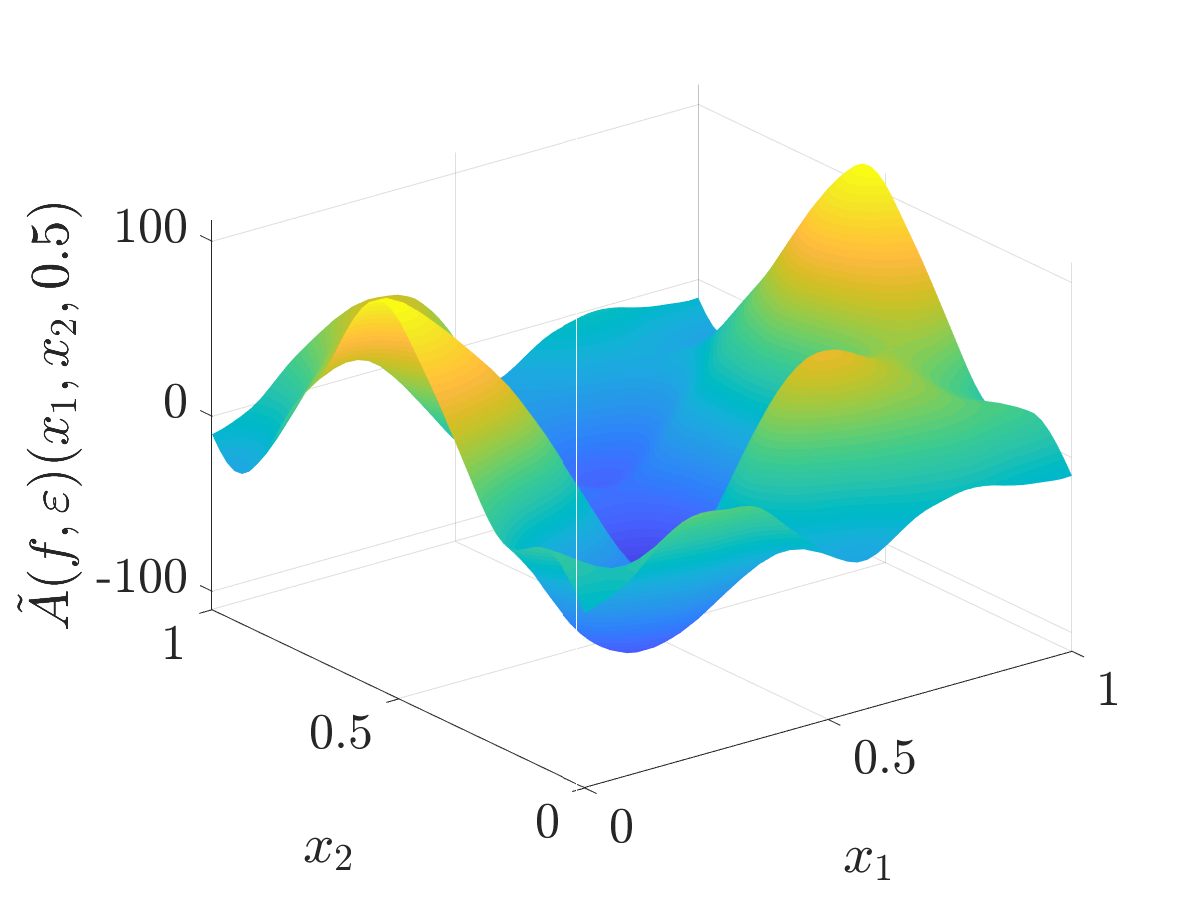
\includegraphics[width =5.5 cm]{ProgramsImages/SimDirectSolAppx.eps} &
		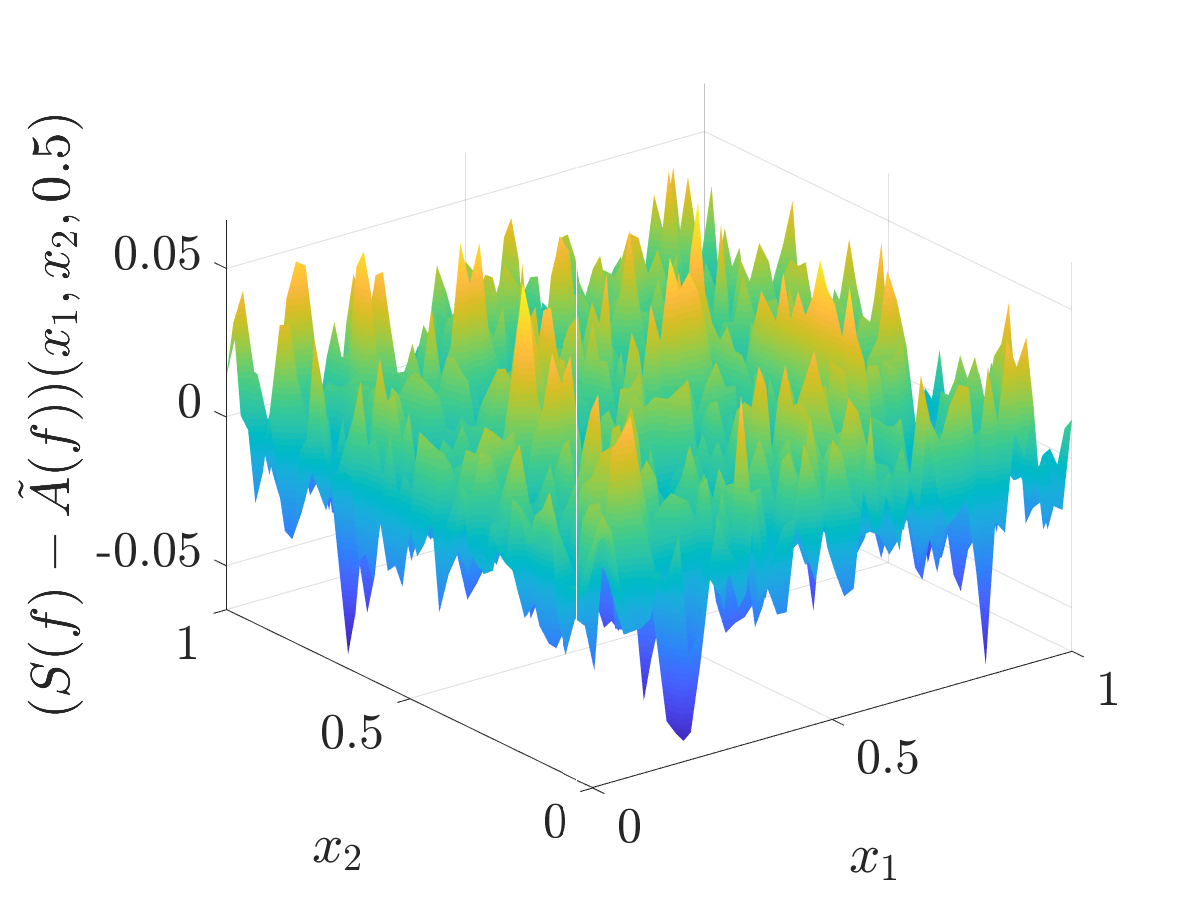
\includegraphics[width = 5.5 cm]{ProgramsImages/SimDirectSolErr.eps}
		\\ (a) & (b)
	\end{tabular}
	\caption{(a) The approximation of the first partial derivative of $f$
		(b) The error of the approximation 
		\label{solfig}} % 
\end{figure}

To do the simulation, we choose the Fourier coefficients $\hf$ to be normal distributed. Let $d=3, a= 2, b=\frac{1}{2},$ and $\varepsilon = 0.1.$ Based on our algorithm, we obtain $ n_{j^\dagger} = 1024.$ Using that, we can obtain the approximated solution and error in Figure \ref{solfig}. Based on Figure \ref{solfig}(b), we can obtain the exact errors are less than $0.01 < \varepsilon $.  This shows our algorithm works.

\begin{figure}[ht]
	\centering
	\begin{tabular}{cc}
		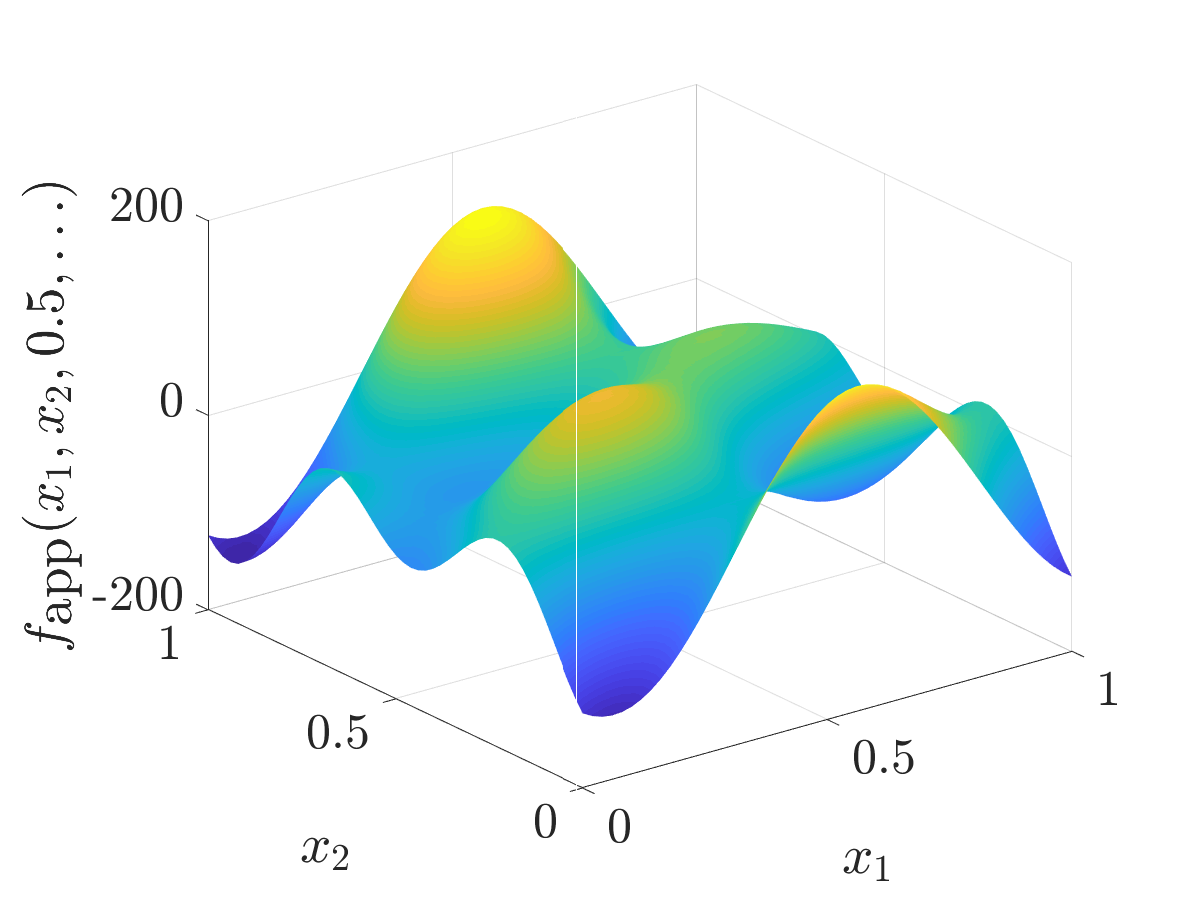
\includegraphics[width = 5.5 cm]{ProgramsImages/SimDirectInpFunAppx.eps}& 
		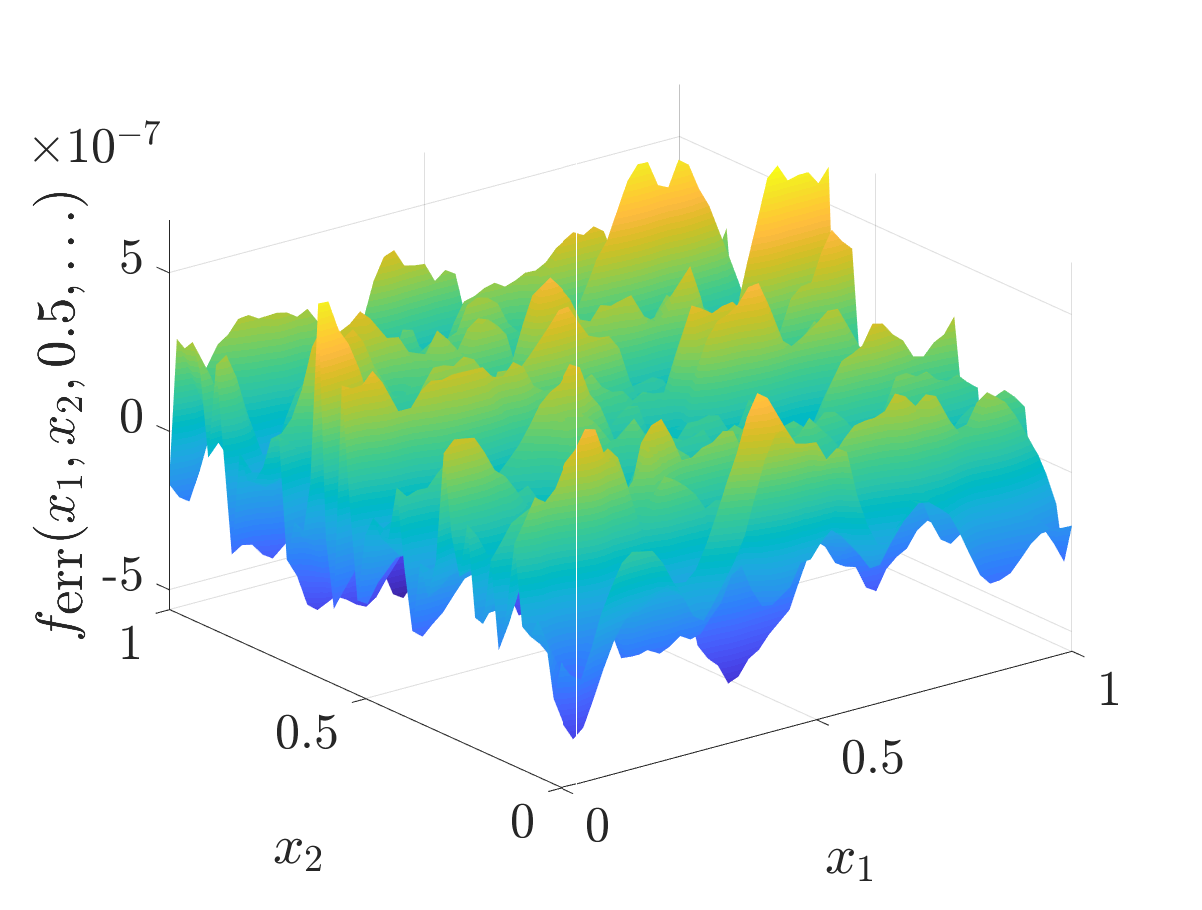
\includegraphics[width = 5.5 cm]{ProgramsImages/SimDirectInpFunErr.eps}
		\\ (a) & (b)
	\end{tabular}
	\caption{(a) The approximation of the input function $f$
		(b) The error of the approximation 
		\label{inpfig}} % 
\end{figure}

Actually, we can also use these 1024 Fourier coefficients to approximate the input function. The above is the approximation of the input function $f$. Notice that, the errors in Figure \ref{inpfig}(b) are much smaller than the errors in Figure \ref{solfig}(b). 


%\subsection{Examples: Approximating the divergence of a vector field}
%
%In this case, $\cf=\{f:\reals^n\mapsto\reals^m,\, f\in C^1(\Omega)\}$ and $\cg=\{g:\reals^n\mapsto\reals,\, g\in C^0(\Omega)\}$ and $S: f\mapsto \nabla\cdot f=\sum_{j=1}^{m}\partial_{x_j}f_j$.
%
%\begin{gather*}
%\norm[\cf]{f} =\left[\int_\Omega \sum_{j=1}^{m}\abs{f_j(x)}^2+\sum_{j=1}^{m}\abs{f'_j(x)}^2 \, \dif x \right]^{1/2},\\
%\norm[\cg]{g} = \left[\int_\Omega \abs{g(x)}^2 \, \dif x \right]^{1/2}, \\
%u_{i}(x) = \frac{\me^{2 \pi \sqrt{-1} <i,x>}}{\sqrt{mV(\omega)+4\pi<i,i>}}, \\
%v_i(x) = \me^{2 \pi \sqrt{-1} <i,x>},\\
% \lambda_i=\frac{2\pi\sqrt{-1}\sum_{j=1}^{m}i_j}{\sqrt{mV(\omega)+4\pi<i,i>}}, \qquad i \in \integers^m,\\
%\pin=\pout=2,\quad q=\infty.
%\end{gather*}

\section{Discussion and Conclusions} \label{sec:conc}

\section*{References}
%\nocite{*}
\bibliographystyle{elsarticle-num}
\bibliography{FJH23,FJHown23}


\end{document}






\begin{rem}
For the algorithm, $\tA$, defined in Algorithm \ref{algo2}, $\cost(\tA,\rho,\varepsilon) \le n_{j^*}$, where $j^*$ satisfies the following upper bound:
\[
j^* \le \min \left \{j \in \naturals : \rho^2 \le \frac{\varepsilon^2(1 - b^2)}{a^2b^2C_{\up}^2n_0^{2(1-p)}} \left[ \frac{1-b^2}{a^2b^{2(j-1)}}+ \frac{1}{2^{2(j-1)(1-p)}}\right]\right\}.
\]
\end{rem}


\begin{proof}
First, we have a rough upper bound on $\cost(\tA,\rho,\varepsilon)$ in the proof of  Theorem  \ref{thm:compcost} by finding the smallest $j$ violating the following inequality:
\begin{equation*}
\rho \ge \norm[\cf]{f} \ge \bignorm[2]{\big( \hf_i \big)_{i=n_{j-1}+1}^{n_j}} \ge \frac{\sigma_j(f)}{\lambda_{n_{j-1}+1}} > \frac{\varepsilon\sqrt{1 - b^2}}{ab \lambda_{n_{j-1}+1}}
\end{equation*}
If we consider $\lambda_{i}$ is bounded above
\begin{equation} \label{lambdaDecI}
\lambda_i \le C_{\up} i^{1-p}, \quad   i \in \naturals,
\end{equation}
where $p > 1$, we obtain
\begin{align*}
\rho & > \frac{\varepsilon\sqrt{1 - b^2}}{ab \lambda_{n_{j-1}+1}} \\
& \ge \frac{\varepsilon\sqrt{1 - b^2}}{ab C_{\up}(n_{j-1}+1)^{1-p}} \qquad \text{by \eqref{lambdaDecI}} \\
& > \frac{\varepsilon\sqrt{1 - b^2}}{ab C_{\up}n_{j-1}^{1-p}} \\
& \ge \frac{\varepsilon\sqrt{1 - b^2}}{ab C_{\up}(2^{j-1}n_0)^{1-p}} \qquad \text{by \eqref{geonj}} \\
& = \frac{\varepsilon\sqrt{1 - b^2}}{ab C_{\up}n_0^{1-p} 2^{(j-1)(1-p)}}
\end{align*}
Thus, one upper bound on $j^*$ is the smallest $j$ violating the above inequality:
\[
j^* \le \min \left \{j \in \naturals :  
j \ge \frac{\log\left[\frac{\varepsilon \sqrt{1-b^2}}{\rho ab C_{\up}n_0^{1-p}}\right]}{(1-p)\log 2}+ 1\right\}
\]

We could also obtain another upper bound similar to the tighter upper bound in Theorem \ref{thm:compcost}.  
The tighter cost is the smallest $j$ that violates the following inequality
\begin{equation*}
\rho^2 > \frac{\varepsilon^2(1 - b^2)}{a^2b^2} \left[ \sum_{k=1}^{j-1} \frac{ b^{2(k-j)}}{a^{2}\lambda_{n_{k-1}+1}^2} + \frac{1}{\lambda_{n_{j-1}+1}^2}\right].
\end{equation*}
From \eqref{lambdaDecI}, we can obtain for any $k=1, \ldots,j-1$
\[\lambda_{n_{k-1}+1} \le C_{\up}(n_{k-1}+1)^{1-p} 
<  C_{\up}(n_{k-1})^{1-p} < C_{\up}n_0^{1-p}.\]
Thus, we have 
\begin{align*}
\rho^2 &> \frac{\varepsilon^2(1 - b^2)}{a^2b^2} \left[ \sum_{k=1}^{j-1} \frac{ b^{2(k-j)}}{a^{2}\lambda_{n_{k-1}+1}^2} + \frac{1}{\lambda_{n_{j-1}+1}^2}\right]\\
& >  \frac{\varepsilon^2(1 - b^2)}{a^2b^2} \left[ \sum_{k=1}^{j-1} \frac{ b^{2(k-j)}}{a^{2}(C_{\up}n_0^{1-p})^2} + \frac{1}{(C_{\up}(n_{j-1})^{1-p} )^2}\right] \\
& = \frac{\varepsilon^2(1 - b^2)}{a^2b^2} \left[ \sum_{k=1}^{j-1} \frac{ b^{2(k-j)}}{a^{2}C_{\up}^2n_0^{2(1-p)}} + \frac{1}{C^2_{\up}(2^{j-1}n_0)^{2(1-p)}}\right] \qquad \text{by \eqref{geonj}}\\
&  =\frac{\varepsilon^2(1 - b^2)}{a^2b^2C_{\up}^2n_0^{2(1-p)}} \left[ \frac{1}{a^2b^{2j}}\sum_{k=1}^{j-1} b^{2k }+ \frac{1}{2^{2(j-1)(1-p)}}\right] \\
& > \frac{\varepsilon^2(1 - b^2)}{a^2b^2C_{\up}^2n_0^{2(1-p)}} \left[ \frac{1-b^2}{a^2b^{2(j-1)}}+ \frac{1}{2^{2(j-1)(1-p)}}\right] .
\end{align*}
Hence, any $j$ that violates the above inequality, must satisfy $j \ge j^*$.
\end{proof}




/fi
\iffalse
\subsection{The embedding of $f(x)=\frac{(b^2-1)}{b^2+1-2b\cos(2\pi x)}$}

In our example, consider $\cf=\cg=\cl_2[0,1]$, and $S: f \mapsto f$ the embedding operator with:
\begin{gather*}
\norm[\cf]{f} = \norm[\cg]{f} = \left[\int_0^1 \abs{f(x)}^2 \, \dif x \right]^{1/2}, \\
u_{i}(x) = v_i(x) = \me^{2 \pi \sqrt{-1} i x},\quad \lambda_i=1, \qquad i \in \integers,\\
\pin=\pout=2,\quad q=\infty.
\end{gather*}

For our index set $\ci=\integers=\{0,1,-1,2,-2,\ldots\}$,
\begin{gather*}
i_j=(-1)^{j}\left\lfloor\frac{j}{2}\right\rfloor,\qquad j\in\naturals,\\
n_0=0,\quad n_k=2k+1, \qquad k\in\naturals.
\end{gather*}

The Fourier coefficients of this function can be easily found:
\begin{align*}
f(x)&=\frac{b^2-1}{b^2+1-2b\cos(2\pi x)}\\
&=\frac{1-b^{-2}+b^{-1}(\me^{-2\pi\sqrt{-1}x}-\me^{-2\pi\sqrt{-1}x})}{1+b^{-2}-b^{-1}(\me^{2\pi\sqrt{-1}x}+\me^{-2\pi\sqrt{-1}x})}\\
&=\frac{(1-b^{-1}\me^{-2\pi\sqrt{-1}x})+(1-b^{-1}\me^{2\pi\sqrt{-1}x})b^{-1}\me^{-2\pi\sqrt{-1}x}}{(1-b^{-1}\me^{2\pi\sqrt{-1}x})(1-b^{-1}\me^{-2\pi\sqrt{-1}x})}\\
&=\frac{1}{1-b^{-1}\me^{2\pi\sqrt{-1}x}}+\frac{b^{-1}\me^{-2\pi\sqrt{-1}x}}{1-b^{-1}\me^{-2\pi\sqrt{-1}x}}\\
&=\sum_{k\in\naturals_0}\left(b^{-1}\me^{2\pi\sqrt{-1}x}\right)^k+\sum_{k\in\naturals}\left(b^{-1}\me^{-2\pi\sqrt{-1}x}\right)^k\\
&=\sum_{k\in\integers}b^{-\abs{k}}\me^{2\pi\sqrt{-1}kx}\Longrightarrow\hf_{i_j}=b^{-\abs{i_j}}
\end{align*}

Because we are interested in seeing how far the approximation is from the real solution, the norm of the exact solution has to be found. Knowing the Fourier coefficients leads us to an easy way to calculate it:
\begin{align*}
\norm[\cg]{S(f)}&=\left(\sum_{j\in\integers}\lambda_{i_j}^2\hf_{i_j}^2\right)^{\frac{1}{2}} =\left(1+2\sum_{k\in\naturals}b^{-2k}\right)^{\frac{1}{2}}=\left(\frac{b^2+1}{b^2-1}\right)^{\frac{1}{2}}
\end{align*}

We can also give the sums of coefficients,
\begin{align*}
&\sigma_1(f)=\sqrt{1+2b^{-2}}\\
&\sigma_k(f)=\sqrt{2}b^{-k}, \qquad k \in\naturals\setminus\{1\}.
\end{align*}
Recalling the alternative definition of the cone in (\ref{decayconedef}), with these sums, $f\in\cc$ for $\gamma_r=b^{-r}$ since
\begin{equation*}
\sigma_k(f) \le \min_{1 \le i <k}\{\gamma_i\sigma_{k-i}(f)\}=\min\left\{1 \; , \; \sqrt{1+\frac{b^2}{2}} \right\}\sigma_k(f)
\end{equation*}

In this case, $\norm[\pout]{\bgamma}=\frac{1}{\sqrt{b^2-1}}$. If we use our Algorithm \ref{algo2}, we have to check first whether $\sqrt{\frac{b^2+2}{b^4-b^2}}\le\varepsilon$. If this inequality states, then $k^*=1$. If not,
\begin{equation*}
k^*=\min\left\{k\in\naturals\setminus\{1\}:\frac{1}{2\log(b)}\log\left(\frac{2}{(b^2-1)\varepsilon^2}\right) \le k \right\}
\end{equation*}

For a numerical application, set $b=3$ and find below a table of results for this example,

\begin{center}
\begin{tabular}{|c|c|c|c|}
  \hline
  % after \\: \hline or \cline{col1-col2} \cline{col3-col4} ...
  $\varepsilon$ & $k^*$ & $n_{k^*}$ & $\operatorname{error}=\norm[\cg]{S(f)}-\norm[\cg]{A_{n_{k^*}}(f)}$ \\
  \hline
  $1$ & $1$ & $3$ & $1.2492\cdot10^{-2}$ \\
  $10^{-1}$ & $2$ & $5$ & $1.3811\cdot10^{-3}$ \\
  $10^{-2}$ & $4$ & $9$ & $1.7041\cdot10^{-5}$ \\
  $10^{-3}$ & $6$ & $13$ & $2.1038\cdot10^{-7}$ \\
  $10^{-4}$ & $8$ & $17$ & $2.5973\cdot10^{-9}$ \\
  $10^{-5}$ & $10$ & $21$ & $3.2065\cdot10^{-11}$ \\
  $10^{-6}$ & $12$ & $25$ & $3.9591\cdot10^{-13}$ \\
  $10^{-7}$ & $15$ & $31$ & $4.4409\cdot10^{-16}$ \\
  \hline
\end{tabular}
\end{center}

\subsection{Derivation of the Bernoulli polynomials}

The properties we will use for these particular polynomials can be found in \cite{AbrSte64}: derivatives, explicit Fourier coefficients, etc. To deal with this example, now $\cf=\cg=\cl_2[0,1]$, and $S: f \mapsto f'$ with,
\begin{gather*}
\norm[\cf]{f} = \left[\int_0^1 \left\{\abs{f(x)}^2 + \abs{f'(x)}^2\right\}\, \dif x\right]^{1/2}, \quad \norm[\cg]{f} = \left[\int_0^1 \abs{f(x)}^2 \, \dif x \right]^{1/2}, \\
u_{i}(x) = \frac{\me^{2 \pi \sqrt{-1} i x}}{\sqrt{1+4 \pi^2 i^2}}, \quad v_i(x) = \me^{2 \pi \sqrt{-1} i x}, \quad \lambda_i=\frac{2 \pi \sqrt{-1} i}{\sqrt{1+4 \pi^2 i^2}}, \qquad i \in \integers,\\
\pin=\pout=2,\quad q=\infty.
\end{gather*}

Like in the previous example, the index set $\ci=\integers=\{0,1,-1,2,-2,\ldots\}$ has the following ordering
\begin{gather*}
i_j=(-1)^{j}\left\lfloor\frac{j}{2}\right\rfloor,\qquad j\in\naturals,\\
n_0=0,\quad n_k=2^k, \qquad k\in\naturals.
\end{gather*}

For this case,
\begin{equation*}
B_n(x)=-\frac{n!}{(2\pi\sqrt{-1})^n}\sum_{k\in\integers\setminus\{0\}}\frac{\me^{2\pi\sqrt{-1}kx}}{k^n}\Longrightarrow
\left\{\begin{array}{l}
\widehat{B_n}_0=0 \\
\widehat{B_n}_{i_j}=-\frac{n!\sqrt{1+4 \pi^2 i_j^2}}{(2\pi\sqrt{-1}i_j)^n},\quad i_j\in\integers\setminus\{0\}
\end{array}\right.
\end{equation*}

Using that $B'_n(x)=nB_{n-1}(x)$ and $\int_0^1B_n(t)B_m(t)\dif t=(-1)^{n-1}\frac{m!n!}{(m+n)!}B_{n+m}$, the real solution comes automatically,
\begin{equation*}
\norm[\cg]{S(B_n(x))}=n\norm[\cg]{B_{n-1}(x)}=n!\sqrt{\frac{\abs{B_{2(n-1)}}}{[2(n-1)]!}}
\end{equation*}
where $B_n=B_n(0)$ are the Bernoulli numbers.

If we consider $\gamma_r=s_1s_2^{-r}$ and that
\begin{equation}\label{bound}
\frac{n!}{\sqrt{2}\pi^n}j^{-n} \le \abs{\lambda_{i_j}\widehat{B_n}_{i_j}} \le \frac{n!2^n}{\pi^n}j^{-n},\quad j\in\naturals\setminus\{1\}
\end{equation}
then $C_{\up}=2^{n+\frac{1}{2}}C_{\lo}=\frac{n!2^n}{\pi^n}$. Thus, as shown in the example example at the beginning of this section we can take
\begin{equation*}
s_1=2\times11^{n-\frac{1}{2}},\quad s_2=2^{n-\frac{1}{2}}
\end{equation*}
There is still one thing to check because $j=1$ was not taken into account in the inequality (\ref{bound}). However, see that $\sigma_1(f) \ge C_{\lo}\left(\frac{5}{36}\right)^{n-\frac{1}{2}}$ what means that the $\gamma_r=s_1s_2^{-r}$ found satisfies our needs.

For a numerical application, find below the results for the case $n=5$ and $n=10$,

\begin{center}
\begin{tabular}{|c|c|c|c|}
  \hline
  % after \\: \hline or \cline{col1-col2} \cline{col3-col4} ...
  \multicolumn{4}{|c|}{$B_5(x)=x^5-\frac{5}{2}x^4+\frac{5}{3}x^3-\frac{1}{6}x$} \\
  \hline
  $\varepsilon$ & $k^*$ & $n_{k^*}$ & $\operatorname{error}=\norm[\cg]{S(B_5(x))}-\norm[\cg]{A_{n_{k^*}}(B_5(x))}$ \\
  \hline
  $1$ & $5$ & $32$ & $2.9439\cdot10^{-11}$ \\
  $10^{-1}$ & $6$ & $64$ & $2.2703\cdot10^{-13}$ \\
  $10^{-2}$ & $7$ & $128$ & $1.8735\cdot10^{-15}$ \\
  $10^{-3}$ & $7$ & $128$ & $1.8735\cdot10^{-15}$ \\
  $10^{-4}$ & $8$ & $256$ & $1.1102\cdot10^{-16}$ \\
  $10^{-5}$ & $9$ & $512$ & $9.7145\cdot10^{-17}$ \\
  \hline
\end{tabular}
\end{center}

\begin{center}
\begin{tabular}{|c|c|c|c|}
  \hline
  % after \\: \hline or \cline{col1-col2} \cline{col3-col4} ...
  \multicolumn{4}{|c|}{$B_{10}(x)=x^{10}-5x^9+\frac{15}{2}x^8-7x^6+5x^4-\frac{3}{2}x^2+\frac{5}{66}$} \\
  \hline
  $\varepsilon$ & $k^*$ & $n_{k^*}$ & $\operatorname{error}=\norm[\cg]{S(B_{10}(x))}-\norm[\cg]{A_{n_{k^*}}(B_{10}(x))}$ \\
  \hline
  $1$ & $5$ & $32$ & $7.7716\cdot10^{-16}$ \\
  $10^{-1}$ & $5$ & $32$ & $7.7716\cdot10^{-16}$ \\
  $10^{-2}$ & $6$ & $64$ & $7.7716\cdot10^{-16}$ \\
  $10^{-3}$ & $6$ & $64$ & $7.7716\cdot10^{-16}$ \\
  $10^{-4}$ & $7$ & $128$ & $7.7716\cdot10^{-16}$ \\
  $10^{-5}$ & $7$ & $128$ & $7.7716\cdot10^{-16}$ \\
  \hline
\end{tabular}
\end{center}

\begin{rem}
MATLAB's machine epsilon is $2.2204\cdot10^{-16}$.
\end{rem}
\fi




\iffalse

We do not expect the series coefficients of the solution $S(f)$, to decay monotonically.  The sequence $\vn$ is used to average finite sequences of Fourier coefficients into groups to smooth the peaks we could encounter if we take these coefficients one by one. Flattening the peaks is a must to fit functions into the cone. Nevertheless, the solution of our algorithm is in this set $\cn$ which means that the sequence does not have to distance the optimal number of data needed in our algorithm (defined below) more than a constant.

We define the optimal number of data needed to solve the problem defined as \eqref{errCond} is 
\begin{equation*}
N_{\opt}(f,\varepsilon)=\min\left\{n\in\naturals:\,\norm[2]{\left(\lambda_{i_j} \hf_{i_j} \right)_{j\ge n+1}} \le \varepsilon \right\}
\end{equation*}

Any algorithm is called \emph{asymptotically  optimal} if it essentially tracks the optimal number of data needed,
\begin{equation} \label{nearoptdef}
\sup_{\varepsilon > 0 } \frac{\cost(A,f;\varepsilon)} {N_{\opt}(f,\varepsilon)} <\infty 
\end{equation}
or
\[
\sup_{\varepsilon > 0 } [\cost(A,f;\varepsilon)- N_{\opt}(f,\varepsilon)] <\infty.
\]

Next, we prove our algorithm is optimal.

\begin{theorem}\label{nopt}
Algorithm \ref{algo2} is optimal for this problem.

\end{theorem}
\begin{proof}
Given $f \in \cc$ and $\varepsilon$, denote $n^*= N_{\opt}(f,\varepsilon)$. Let 
\[n_{k^*-r-1} < n^{*}  \le n_{k^*-r} \le n_{k^*},\]
where $n_{k^*}$ is the cost of our algorithm.
Thus by \eqref{sumdef}, we obtain
\[\sigma_{k^*-r+1}(f) = \norm[2]{ \left(\lambda_{i_j} \hf_{i_j} \right)_{j=n_{k^*-r}+1}^{n_{k^*-r+1}}}
 \le \norm[2]{ \left(\lambda_{i_j} \hf_{i_j} \right)_{j=n^*}^{\infty}} \le \varepsilon.\]
By the cone condition \eqref{decayconedef} , we have 
\[\sigma_{k^*-r+m}(f) \le \gamma_{m-1}\sigma_{k^*-r+1}(f) \le\gamma_{m-1} \cdot \varepsilon.\]
Choose $m$ such that $\gamma_{m-1} \le \frac{1}{\norm[2]{\vgamma}},$
thus we obtain
\[\sigma_{k^*-r+m}(f) \le\gamma_{m-1} \cdot \varepsilon \le \frac{\varepsilon}{\norm[2]{\vgamma}}.\]
Suppose $\gamma_r$ decays geometrically, $n_k$ increases geometrically $n_k = n_0 2^k $, we have
\[\frac{\cost(\tA,f;\varepsilon)}{N_{\opt}(f,\varepsilon)} \le 
\frac{n_{k^*-r+m}}{n_{k^*-r-1}} = \frac{n_0 2^{k^*-r+m}}{n_0 2^{k^*-r-1}}
= 2^{m+1}.\]


As $m$ satisfied 
\begin{align*}\
\gamma_{m-1} \le \frac{1}{\norm[2]{\vgamma}} 
& \Longleftrightarrow C_1C_2^{-m+1} \le \frac{\sqrt{C_2^2-1}}{C_1} \\
& \Longrightarrow C_2^{-m+1} \le \frac{\sqrt{C_2^2-1}}{C^2_1} \\
& \Longrightarrow  m \ge 1+ 
\frac{\log\left(\frac{C_1^2}{\sqrt{C_2^2-1}}\right)}{\log(C_2)}.
\end{align*}
Therefore we can choose 
\[m = \left\lceil 1+ 
\frac{\log\left(\frac{C_1^2}{\sqrt{C_2^2-1}}\right)}{\log(C_2)} \right\rceil
 < 2 + \frac{\log\left(\frac{C_1^2}{\sqrt{C_2^2-1}}\right)}{\log(C_2)}. \]
Hence,
 \[\frac{\cost(A,f;\varepsilon)} {N_{\opt}(f,\varepsilon)} 
 \le 2^{m+1} < 2^{3+\frac{\log\left(\frac{C_1^2}{\sqrt{C_2^2-1}}\right)}{\log(C_2)}} \Longrightarrow \sup_{f,\varepsilon} \frac{\cost(A,f;\varepsilon)} {N_{\opt}(f,\varepsilon)} <\infty.\]

Suppose $\gamma_r$ decays geometrically, $n_k$ increases linearly $n_k = n_0 + 2k $, we have
\begin{align*}
\cost(\tA,f;\varepsilon)-N_{\opt}(f,\varepsilon) & \le 
n_{k^*-r+m}-n_{k^*-r-1} \\ & = (n_0 +2(k^*-r+m))-(n_0+2(k^*-r-1))\\
& = 2(m+1).
\end{align*}
Still choose
\[m = \left\lceil 1+ 
\frac{\log\left(\frac{C_1^2}{\sqrt{C_2^2-1}}\right)}{\log(C_2)} \right\rceil
 < 2 + \frac{\log\left(\frac{C_1^2}{\sqrt{C_2^2-1}}\right)}{\log(C_2)}. \]
 We have
\begin{align*}
\cost(\tA,f;\varepsilon)-N_{\opt}(f,\varepsilon) 
& = 2(m+1) \\
&  = 2\left(3+ \frac{\log\left(\frac{C_1^2}{\sqrt{C_2^2-1}}\right)}{\log(C_2)}\right)\\
\Longrightarrow &
\sup_{f,\varepsilon} \left[\cost(A,f;\varepsilon) -N_{\opt}(f,\varepsilon) \right]< \infty
\end{align*}
\end{proof}

\fi


